\documentclass[aspectratio=169]{beamer}

\usetheme{Boadilla}
\usefonttheme{professionalfonts}
\setbeamertemplate{navigation symbols}{}
\setbeamertemplate{itemize items}[circle]
\setbeamertemplate{enumerate items}[default]
\setbeamertemplate{headline}{}

\usepackage[utf8]{inputenc}
\usepackage[T1]{fontenc}
\usepackage{lmodern}
\usepackage{amsmath}
\usepackage{booktabs}
\usepackage{tabularx}
\usepackage{array}
\usepackage{hyperref}
\usepackage[strings]{underscore}
\usepackage{listings}
\usepackage{tikz}
\usetikzlibrary{arrows.meta,positioning,fit,calc,shapes.geometric}
\usepackage{xcolor}

\definecolor{courseblue}{HTML}{12355B}
\definecolor{coursegold}{HTML}{C98A2E}
\definecolor{courseice}{HTML}{EEF3F8}
\definecolor{coursegreen}{HTML}{2F6B4F}
\definecolor{coursegray}{HTML}{4B5563}
\definecolor{codebg}{HTML}{F7F9FC}
\definecolor{codecomment}{HTML}{5E6C84}
\definecolor{codestring}{HTML}{0B6E4F}

\setbeamercolor{palette primary}{bg=courseblue,fg=white}
\setbeamercolor{palette secondary}{bg=coursegold,fg=white}
\setbeamercolor{palette tertiary}{bg=courseblue,fg=white}
\setbeamercolor{palette quaternary}{bg=coursegold,fg=white}
\setbeamercolor{structure}{fg=courseblue}
\setbeamercolor{frametitle}{bg=courseice,fg=courseblue}
\setbeamercolor{title}{fg=courseblue}
\setbeamercolor{block title}{bg=courseblue,fg=white}
\setbeamercolor{block body}{bg=courseice,fg=black}
\setbeamercolor{normal text}{fg=black,bg=white}
\setbeamercolor{alerted text}{fg=coursegold}

\setbeamerfont{footline}{size=\scriptsize}

\setbeamertemplate{footline}{
  \leavevmode
  \hbox{
    \begin{beamercolorbox}[wd=.33\paperwidth,ht=2.8ex,dp=1.2ex,leftskip=0.8em]{palette primary}%
      University of Trieste
    \end{beamercolorbox}%
    \begin{beamercolorbox}[wd=.49\paperwidth,ht=2.8ex,dp=1.2ex,center]{palette tertiary}%
      \coursename{} \textbar{} \coursecode
    \end{beamercolorbox}%
    \begin{beamercolorbox}[wd=.18\paperwidth,ht=2.8ex,dp=1.2ex,rightskip=0.8em plus1fil]{palette secondary}%
      \insertframenumber{} / \inserttotalframenumber
    \end{beamercolorbox}%
  }
}

\hypersetup{
  colorlinks=true,
  linkcolor=courseblue,
  urlcolor=coursegreen
}

\lstdefinestyle{coursepython}{
  language=Python,
  basicstyle=\ttfamily\footnotesize,
  keywordstyle=\color{courseblue}\bfseries,
  commentstyle=\color{codecomment}\itshape,
  stringstyle=\color{codestring},
  showstringspaces=false,
  columns=fullflexible,
  keepspaces=true,
  frame=single,
  framerule=0.6pt,
  rulecolor=\color{courseblue},
  backgroundcolor=\color{codebg},
  xleftmargin=0.4em,
  xrightmargin=0.4em,
  aboveskip=0.4em,
  belowskip=0.2em
}

\newcommand{\coursename}{Data-driven Systems Engineering}
\newcommand{\coursecode}{440MI / 305SM}
\newcommand{\coursefooter}{}

\newcommand{\learninggoals}[1]{
  \begin{block}{Learning goals}
  #1
  \end{block}
}

\newcommand{\repoactivity}[1]{
  \begin{block}{Repo activity}
  #1
  \end{block}
}

\newcommand{\readinglist}[1]{
  \begin{block}{Papers and materials}
  {\footnotesize #1}
  \end{block}
}

\newcommand{\coursecontextframe}[5]{
  \begin{frame}{Course Map and Running Cases}
  \centering
  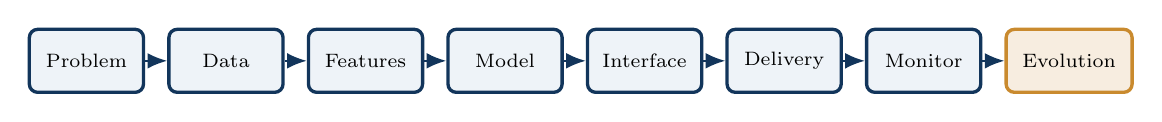
\begin{tikzpicture}[node distance=0.28cm]
  \node[flowbox, minimum width=1.45cm, minimum height=0.8cm] (problem) {\scriptsize Problem};
  \node[flowbox, minimum width=1.45cm, minimum height=0.8cm, right=of problem] (data) {\scriptsize Data};
  \node[flowbox, minimum width=1.45cm, minimum height=0.8cm, right=of data] (features) {\scriptsize Features};
  \node[flowbox, minimum width=1.45cm, minimum height=0.8cm, right=of features] (model) {\scriptsize Model};
  \node[flowbox, minimum width=1.45cm, minimum height=0.8cm, right=of model] (interface) {\scriptsize Interface};
  \node[flowbox, minimum width=1.45cm, minimum height=0.8cm, right=of interface] (delivery) {\scriptsize Delivery};
  \node[flowbox, minimum width=1.45cm, minimum height=0.8cm, right=of delivery] (monitor) {\scriptsize Monitor};
  \node[accentbox, minimum width=1.6cm, minimum height=0.8cm, right=of monitor] (evolution) {\scriptsize Evolution};
  \foreach \a/\b in {problem/data,data/features,features/model,model/interface,interface/delivery,delivery/monitor,monitor/evolution} {
    \draw[arrow] (\a) -- (\b);
  }
  \end{tikzpicture}

  \vspace{0.5em}
  \begin{block}{Today in the course}
  \textbf{Focus:} #1

  \textbf{Bridge:} #2
  \end{block}

  \begin{columns}[T]
  \column{0.48\textwidth}
  \begin{block}{Fraud case}
  {\footnotesize #3}
  \end{block}
  \column{0.48\textwidth}
  \begin{block}{Pasteurization case}
  {\footnotesize #4}
  \end{block}
  \end{columns}

  \vspace{0.3em}
  {\footnotesize \textbf{Course thread:} #5}
  \coursefooter
  \end{frame}
}

\newcommand{\classclosingframe}[4]{
  \begin{frame}{From This Class to the Next}
  \begin{block}{What stays with us}
  #1
  \end{block}

  \begin{columns}[T]
  \column{0.48\textwidth}
  \begin{block}{Project use}
  {\footnotesize #2}
  \end{block}
  \column{0.48\textwidth}
  \begin{block}{Next connection}
  {\footnotesize #3}
  \end{block}
  \end{columns}

  \vspace{0.3em}
  {\footnotesize \textbf{Course thread:} #4}
  \coursefooter
  \end{frame}
}

\tikzset{
  flowbox/.style={
    rounded corners=3pt,
    draw=courseblue,
    fill=courseice,
    very thick,
    minimum width=2.2cm,
    minimum height=0.9cm,
    align=center,
    font=\small
  },
  accentbox/.style={
    rounded corners=3pt,
    draw=coursegold,
    fill=coursegold!15,
    very thick,
    minimum width=2.2cm,
    minimum height=0.9cm,
    align=center,
    font=\small
  },
  arrow/.style={
    -{Latex[length=2.5mm,width=2mm]},
    thick,
    draw=courseblue
  }
}


\title{Class 5: Practice 1 --- Streamlit}
\author{\coursename}
\date{}

\begin{document}

\frame{\titlepage \coursefooter}

\begin{frame}{Agenda}
\begin{itemize}
\item What Streamlit is and why a data course needs it early.
\item Installing Streamlit and running a first script.
\item Reading the real dashboard entry point: `streamlit/Main.py`.
\item Where the fraud model behind that dashboard comes from: `streamlit/modeling.py`.
\item Hands-on practice: two small Streamlit applications.
\end{itemize}
\coursefooter
\end{frame}

\begin{frame}{Learning goals}
\learninggoals{
\begin{itemize}
\item Explain what Streamlit adds on top of a plain Python script.
\item Install Streamlit and run an app locally.
\item Read and modify an existing multi-page Streamlit application.
\item Build a small Streamlit app from user input to computed output.
\item Handle missing or invalid input with clear error and warning messages.
\end{itemize}
}
\coursefooter
\end{frame}

\coursecontextframe
{First hands-on practice: turning a script into an interactive app with Streamlit.}
{Loops, conditionals, functions, and lists from the last two classes now become the logic behind a page someone else can click through.}
{The fraud case's dashboard, `streamlit/Main.py` plus `streamlit/pages/App_Credit_Card.py`, is the app you will run today, not a hypothetical one.}
{The same pattern later serves the pasteurization simulator: a Python script, wrapped in Streamlit, becomes a live monitoring page.}
{From here on, ``the app'' in this course usually means a Streamlit app, and today is where that stops being abstract.}

\begin{frame}{What Streamlit is}
\begin{itemize}
\item An open-source Python library for building interactive web apps, aimed at machine learning and data science.
\item No HTML, CSS, or JavaScript required to get a working interface.
\item A script is re-run top to bottom on every user interaction, which keeps the mental model simple.
\item Good fit for demos, dashboards, and teaching; not a replacement for a full production frontend.
\end{itemize}
\coursefooter
\end{frame}

\begin{frame}{How a Streamlit app is served}
\centering
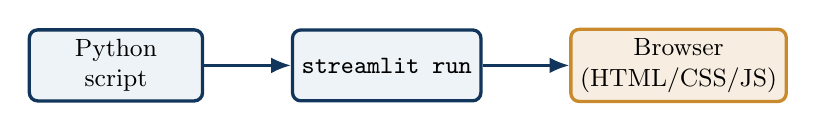
\begin{tikzpicture}[node distance=1.1cm and 1.1cm]
\node[flowbox] (script) {Python\\script};
\node[flowbox, right=of script] (run) {\texttt{streamlit run}};
\node[accentbox, right=of run] (browser) {Browser\\(HTML/CSS/JS)};
\draw[arrow] (script) -- (run);
\draw[arrow] (run) -- (browser);
\end{tikzpicture}
\vspace{0.6em}
\begin{itemize}
\item You write plain Python; Streamlit's client-server layer renders it as a page at \texttt{localhost:8501} by default.
\item Every widget interaction round-trips back to your script and re-executes it.
\end{itemize}
\coursefooter
\end{frame}

\begin{frame}[fragile]{Install and run}
\begin{lstlisting}[style=coursepython]
pip install streamlit
streamlit run Main.py
\end{lstlisting}
\begin{itemize}
\item \texttt{pip install streamlit} adds it to your environment, alongside the other packages in `requirements.txt`.
\item \texttt{streamlit run <file>.py} launches the app and opens it in your default browser.
\item Running it from inside `streamlit/` starts the exact dashboard this course uses.
\end{itemize}
\coursefooter
\end{frame}

\begin{frame}[fragile]{Reading `streamlit/Main.py`}
\begin{lstlisting}[style=coursepython]
st.set_page_config(
    page_title="440MI - Machine Learning Dashboard",
    layout="wide",
    initial_sidebar_state="expanded"
)

st.title("Machine Learning Streamlit Hub")
st.markdown("""
Welcome to the 440MI + 305SM Course.
This interface automatically discovers all available modules
inside the `pages/` directory.
""")
\end{lstlisting}
\begin{itemize}
\item \texttt{set\_page\_config} runs once and configures the whole app; \texttt{title} and \texttt{markdown} render text on the page.
\item Streamlit auto-discovers any script placed in `streamlit/pages/` as a separate page --- that is how `App_Credit_Card.py` gets a sidebar entry with no extra wiring.
\end{itemize}
\coursefooter
\end{frame}

\begin{frame}{Live demo}
\repoactivity{
\begin{itemize}
\item Run \texttt{streamlit run streamlit/Main.py} and open the sidebar to reach \texttt{App\_Credit\_Card}, \texttt{App\_Pasteurization}, and \texttt{App\_Stream}.
\item Move a slider on the fraud page and watch the script re-run: this is the ``re-run top to bottom on interaction'' model from two slides ago, live.
\item No new code is needed for this demo: the app already exists in this repository.
\end{itemize}
}
\coursefooter
\end{frame}

\begin{frame}[fragile]{Where the model behind the app comes from}
\begin{lstlisting}[style=coursepython]
scaler = StandardScaler()
X_train_scaled = scaler.fit_transform(X_train)

cls = RandomForestClassifier(n_estimators=200, random_state=42, n_jobs=-1)
cls.fit(X_train_scaled, y_train)

with open('model.pkl', 'wb') as f:
    pickle.dump(cls, f)
\end{lstlisting}
\begin{itemize}
\item `streamlit/modeling.py` is the script that produces \texttt{model.pkl} and \texttt{scaler.pkl}, the two files the app loads at start-up.
\item You do not need to understand \texttt{RandomForestClassifier} yet --- only that a trained object gets pickled to disk, exactly as any Python object can be.
\end{itemize}
\coursefooter
\end{frame}

\begin{frame}[fragile]{From pickle file to page}
\begin{lstlisting}[style=coursepython]
model = pickle.load(open('model.pkl', 'rb'))
scaler = pickle.load(open('scaler.pkl', 'rb'))

if st.button("Predict Fraud Risk"):
    prediction = model.predict(scaled)[0]
    probability = model.predict_proba(scaled)[0][1]
\end{lstlisting}
\begin{itemize}
\item `App_Credit_Card.py` loads both pickled objects once, then reuses them on every button click.
\item This closes the loop from Class 4: an \texttt{if} guarding a button click, calling a function (\texttt{.predict}) that returns a value.
\end{itemize}
\coursefooter
\end{frame}

\begin{frame}{Practice task 1: descriptive statistics app}
\begin{itemize}
\item Build a Streamlit app that accepts a list of float numbers from the user.
\item Compute and display: mean, standard deviation, minimum, and maximum.
\item Reuse the \texttt{summarize()} function pattern from Class 4 instead of writing the arithmetic inline.
\item Keep the interface to a handful of widgets: one input, four displayed results.
\end{itemize}
\coursefooter
\end{frame}

\begin{frame}{Practice task 2: student grouping app}
\begin{itemize}
\item Input: the number of groups, and a list of student names.
\item Output: the students organized into that many groups.
\item Requirement: every group must have the same number of students.
\item Handle the edge cases explicitly: an error message when there are no students, a warning when group sizes cannot come out even.
\end{itemize}
\coursefooter
\end{frame}

\begin{frame}{A small widget cheat sheet}
\begin{tabularx}{\textwidth}{>{\bfseries}l X}
Widget & Typical use \\
\toprule
\texttt{st.number\_input} / \texttt{st.slider} & Collect a numeric value from the user. \\
\texttt{st.button} & Trigger an action, such as running a prediction. \\
\texttt{st.error} / \texttt{st.warning} / \texttt{st.success} & Give clear, colored feedback on the outcome. \\
\texttt{st.title} / \texttt{st.markdown} & Static text and page structure. \\
\bottomrule
\end{tabularx}
\coursefooter
\end{frame}

\begin{frame}{Discussion prompt}
\begin{block}{Question}
`App_Credit_Card.py` loads \texttt{model.pkl} once at the top of the script, even though the whole script re-runs on every interaction. Why does that matter for performance, and what would happen if loading were inside the button's \texttt{if} block instead?
\end{block}
\begin{itemize}
\item Introduces the idea that where code sits in a re-run model has real cost --- a first, informal step toward the caching concepts used later in the course.
\end{itemize}
\coursefooter
\end{frame}

\begin{frame}{Papers and materials}
\readinglist{
\href{https://docs.streamlit.io/get-started}{Get started with Streamlit};\
\href{https://docs.streamlit.io/}{Streamlit documentation};\
\href{https://scikit-learn.org/stable/}{scikit-learn documentation}.
}
\coursefooter
\end{frame}

\classclosingframe
{\begin{itemize}
\item Streamlit turns a Python script into an interactive page with no separate frontend code.
\item `Main.py`, `modeling.py`, and `App_Credit_Card.py` already show the full path from training to pickle to interface.
\item Practicing on two small apps builds the same muscle needed for the full fraud dashboard.
\end{itemize}}
{If your project needs a quick interface for a stakeholder, Streamlit is very likely the fastest path there.}
{Class 6 goes back one step, to reading and writing files and plotting with pandas and Matplotlib, so the data behind these apps is not always hardcoded.}
{Today's interface needs data; the next class is about getting that data in and visualized.}

\end{document}
